\documentclass{standalone}
\usepackage{xcolor}
\usepackage{verbatim}
\usepackage[T1]{fontenc}
\usepackage{graphics}
\usepackage{hyperref}
\newcommand{\code}[1]{\texttt{#1}}
\newcommand{\R}{R}
\newcommand{\pkg}[1]{#1}
\newcommand{\CRANpkg}[1]{\pkg{#1}}%
\newcommand{\BIOpkg}[1]{\pkg{#1}}
\usepackage{amsmath,amssymb,array}
\usepackage{booktabs}
\providecommand{\tightlist}{%
  \setlength{\itemsep}{0pt}\setlength{\parskip}{0pt}}
\usepackage{color} 
\usepackage{tikz} 
\usepackage{pgfplots} 
\pgfplotsset{compat=1.17} 
\usetikzlibrary{arrows.meta} 
\usepackage{caption} 
\usepackage{amsfonts} 
\usepackage{hyperref} 
\usepackage{threeparttable} 
\usepackage{float} 
\usepackage{amsmath} 
\usepackage{bm} 
\usepackage{booktabs} 
\usepackage{makecell} 
\hypersetup{
  colorlinks=true,
  linkcolor=blue,
  }
\newcommand{\indep}{\perp \!\!\! \perp}

\begin{document}
\nopagecolor
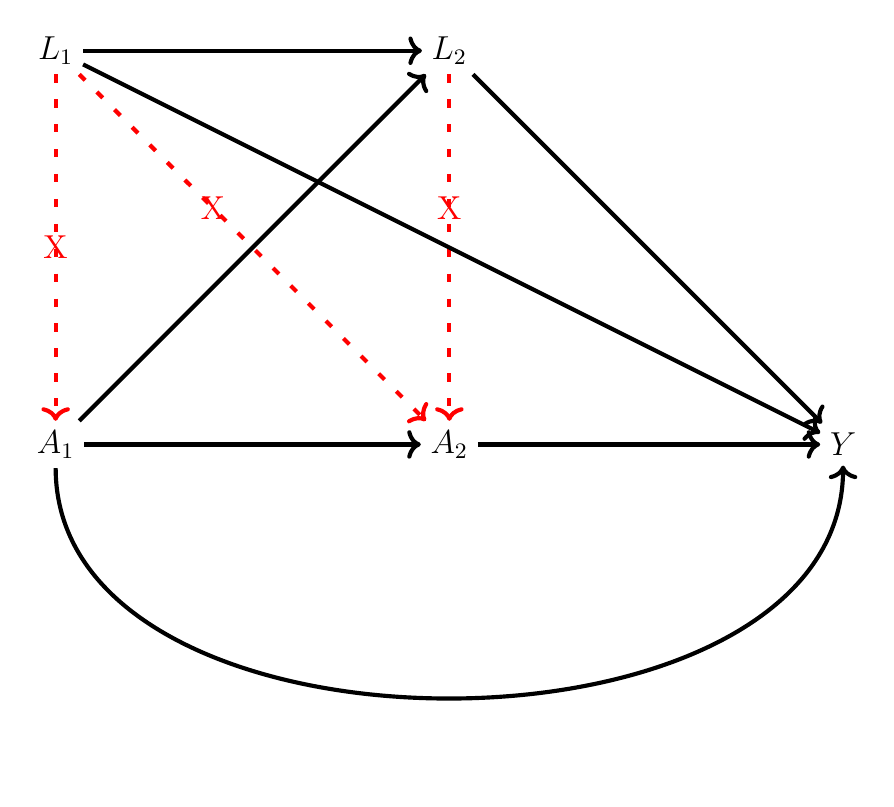
\begin{tikzpicture}
\node (L1) at (0, 0) {\large $L_{1}$};
\node (L2) at (5, 0) {\large $L_{2}$};
\node (A1) at (0, -5) {\large $A_{1}$};
\node (A2) at (5, -5) {\large $A_{2}$};
\node (Y) at (10, -5) {\large $Y$};
\node[red] at (0, -2.5) {\large X};
\node[red] at (5, -2) {\large X};
\node[red] at (2, -2) {\large X};
\draw [->, line width= 1.5] (L1) -- (L2);
\draw [->, red, loosely dashed, line width= 1.5] (L1) -- (A1);
\draw [->, red, loosely dashed, line width= 1.5] (L1) -- (A2);
\draw [->, red, loosely dashed, line width= 1.5] (L2) -- (A2);
\draw [->, line width= 1.5] (A1) -- (A2);
\draw [->, line width= 1.5] (A1) to[out=-90,in=-90] (Y);
\draw [->, line width= 1.5] (A1) -- (L2);
\draw [->, line width= 1.5] (L1) -- (Y);
\draw [->, line width= 1.5] (A2) -- (Y);
\draw [->, line width= 1.5] (L2) -- (Y);
\end{tikzpicture}
\end{document}
